%!TEX program = xelatex
\documentclass[10pt,mathserif]{beamer}%,aspectratio=169 %画面比例16:9%
\usepackage{verbatimbox,color}
\usepackage{picinpar,graphicx}
\usepackage{smartdiagram}
\usesmartdiagramlibrary{additions}
\usepackage{multicol}
\usepackage{biblatex}
\usepackage{xmpmulti}
\usepackage{xeCJK}
\usepackage{hyperref} % links
\usepackage{pgfgantt}
\usepackage{pdfpages}
\usetheme[
 sidebar, xdblue
 ]{XDUstyle}
\usepackage{mdframed} 
\theoremstyle{definition}
\mdfdefinestyle{theoremstyle}{%
	linecolor=gray!40,linewidth=.5pt,%
	backgroundcolor=gray!10,
	skipabove=8pt,
	skipbelow=5pt,
	innerleftmargin=7pt,
	innerrightmargin=7pt,
	frametitlerule=true,%
	frametitlerulewidth=.5pt,
	frametitlebackgroundcolor=gray!15,
	frametitleaboveskip=0pt,
	frametitlebelowskip=0pt,
	innertopmargin=.4\baselineskip,
	innerbottommargin=.4\baselineskip,
	shadow=true,shadowsize=3pt,shadowcolor=black!20,
	theoremseparator={.},
}
%[section]means add the section number in the first place.


\title{题目}
\subtitle{子标题}
\institute[中国科学院大学\\生命科学学院]{指导老师:某某某} % 中括号部分为导航栏底所用尽可能精简
\author{作者:某某}
\date{xxxx年xx月xx日}% 时间可自行设置
	
\begin{document}%
{\xdbg \frame[plain,noframenumbering]{\titlepage}}%首页标题页

%显示目录
\AtBeginSection[]
{
	\begin{frame}[noframenumbering]{目录}
		\tableofcontents[subsectionstyle=hide]
	\end{frame}
	\begin{frame}[noframenumbering]{目录}
		\tableofcontents[currentsection,subsectionstyle=hide]
	\end{frame}
}
\section{第一部分}

\subsection{子标题1.1}
\begin{frame}{\insertsubsection}
	内容......
\end{frame}

\subsection{子标题1.2}
\begin{frame}{\insertsubsection}
	植物物种多样性与微生物多样性的关系
	微生物对植物的影响
		\begin{center}
			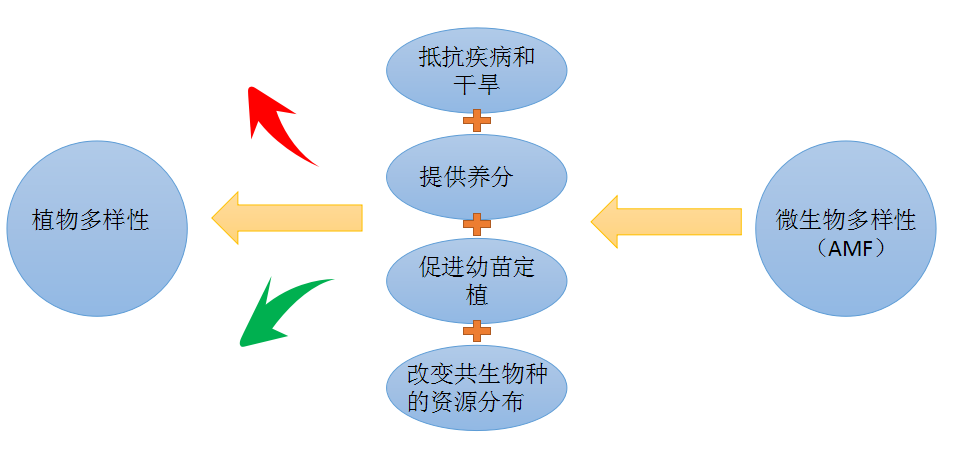
\includegraphics[width = 0.9\textwidth]{./pic/1.2.3.png}
		\end{center}
		(reference; )
\end{frame}

\subsection{子标题1.3}
\begin{frame}{\insertsubsection}
	研究目的
	\begin{itemize}
		\item a
		\item b
		\item c
	\end{itemize}
\end{frame}
\section{第二部分}
\subsection{子标题1.1}
\begin{frame}{\insertsubsection}
	\begin{columns}
		\column{0.35\textwidth}
		常见的研究方法:
		\begin{itemize}
			\item<1-> a
			\item<2-> b		
		\end{itemize}
		\column{0.65\textwidth}
		\begin{center}
			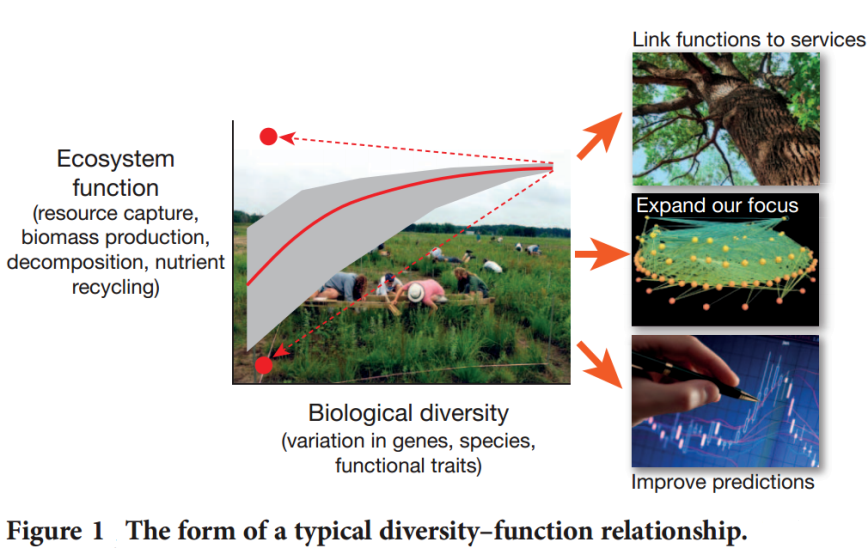
\includegraphics[width = \textwidth]{./pic/2.1.1.png}
		\end{center}
	\end{columns}
\end{frame}


\subsection{子标题2.2}
\begin{frame}{\insertsubsection}
	内容...
\end{frame}



\section{第三部分}
\begin{frame}{\insertsection}{\insertsubsection}
\begin{center}
	\begin{tabular}{ l l  }
		2016.07-2016.10: & 对以往研究进行Meta分析;\\ 
		2016.10-2016.10: & 野外补样;\\
		2016.11-2017.01: & 分析青海样带植物多样性与\\
		& 微生物多样性的关系;\\
		2017.02-2017.06: & 分析西藏样带植多样性与\\
		& 微生物多样性的关系并撰写文章;\\  
		2017.12-2017.12: & 中期答辩\\
		2018.01-2018.03: & 博士学位论文撰写\\
		2018.05-2018.05: & 毕业答辩
	\end{tabular}
\end{center}

\end{frame}
\begin{frame}{\insertsection}{\insertsubsection}
	\begin{center}
		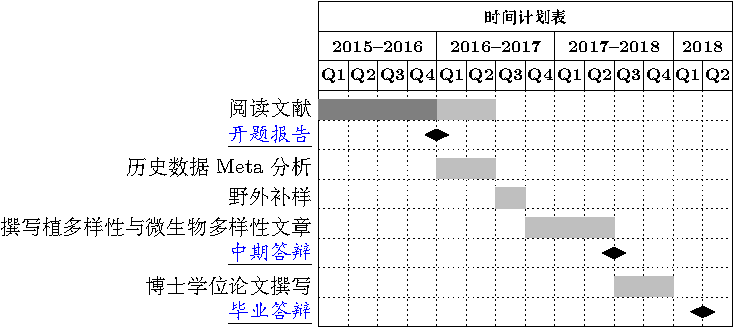
\includegraphics[width = \textwidth]{./pic/gatt.pdf}
	\end{center}
\end{frame}




{\xdbg%末页致谢
\begin{frame}[plain,noframenumbering]
 \finalpage{{\huge 感谢观看!}}
\end{frame}}


\end{document} 
